% Some LaTeX commands I define for my own nomenclature.
% If you have to, it's better to change nomenclature once here than in a 
% million places throughout your thesis!


%======================================================================
\chapter{Literature Review}
\label{c2}
%======================================================================

As people's awareness of disaster prevention has increased in recent years, the number of disaster prevention and evacuation studies has increased year after year. On the other hand, using statistical knowledge to analyze some sociological issues is also one of the popular research directions. This research is a hybrid of the two domains mentioned above. This study focuses on people's evacuation behavior in terms of disasters, to promote a link between the respondents' demographic information elements, prior experiences with travel/evacuation dramas/disasters, and their behavior patterns in disasters. On the other side, the researchers measured how the above characteristics influenced their perceptions of the disaster prevention application called Safety Tips. Therefore, the analysis methods of many sociology-oriented studies for questionnaires, especially those containing scale-based questions, were also referred to. 

After the 2018 Hokkaido Eastern Iburi earthquake, Survey Research Center, Inc. Center, Inc. completed this survey conducted a survey~\cite{ref50} on the evacuation behavior of foreign visitors to Japan. The survey was completed in September 2018,  interviewed 185 foreign tourists visiting Japan who stayed in Hokkaido on September 6, 2018, asking about their behavior during the earthquake, evacuation guidance provided by accommodation facilities, and problems encountered during the earthquake. The survey shows that the inability to access information and charge cell phones due to power outages were the biggest difficulties for foreign visitors. Also, the language barrier makes it difficult to know what to do and to understand the information available locally. Combined with the lack of direct evacuation information available on smartphones and the lack of evacuation guidelines in hotels, these caused significant difficulties for foreign visitors to evacuate shown in Figure~\ref{fig2a}. 

\begin{figure*}[h]
  \begin{subfigure}{\textwidth}
    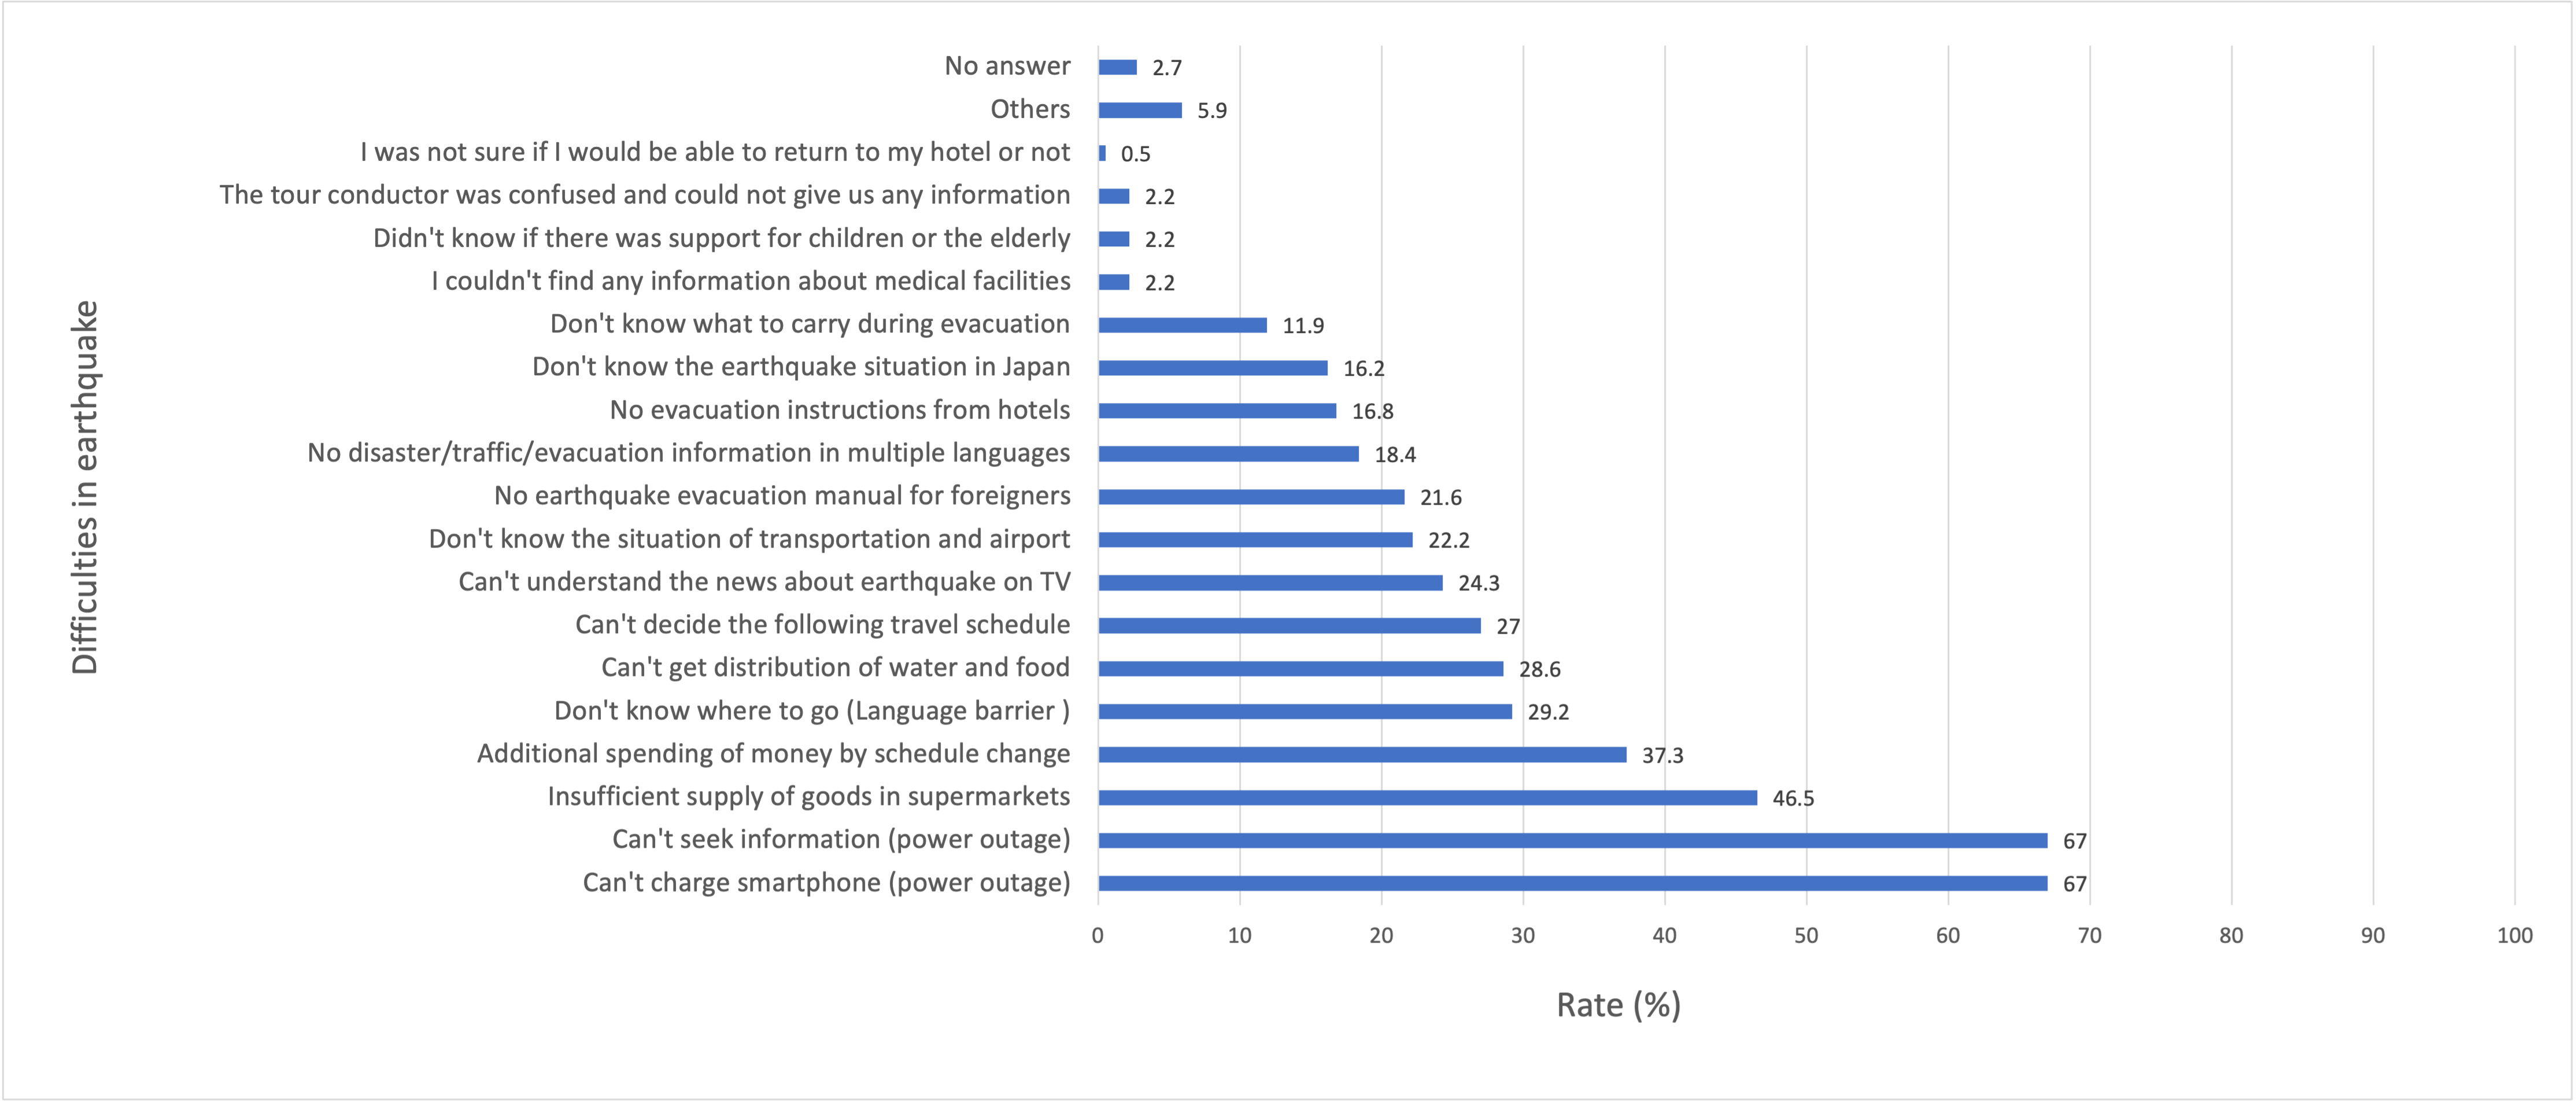
\includegraphics[width=\linewidth]{Figure/Figure2a.png}
    \caption{Difficulties in earthquake}
    \label{fig2a}
  \end{subfigure}
  \begin{subfigure}{\textwidth}
    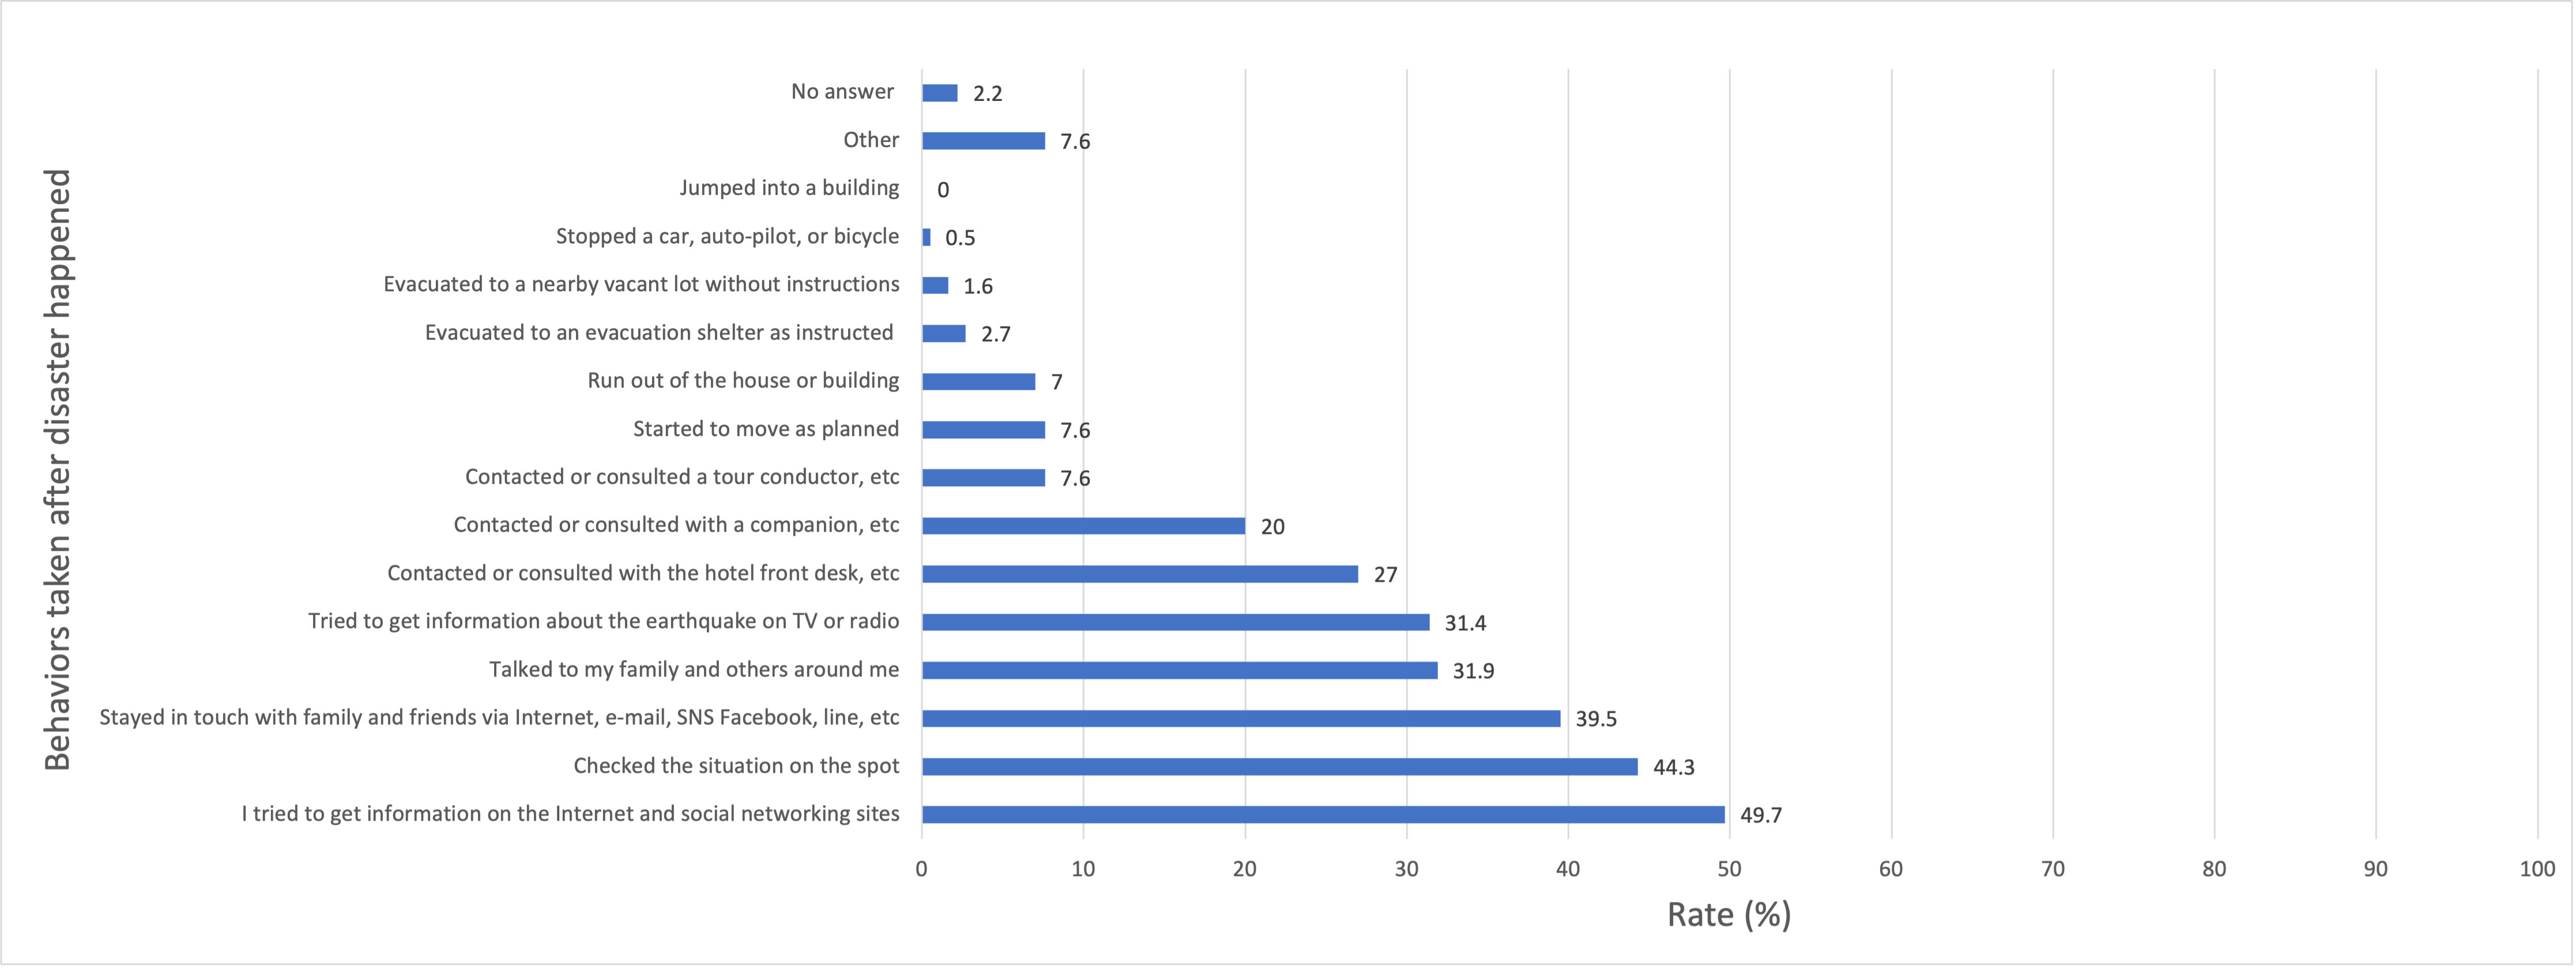
\includegraphics[width=\linewidth]{Figure/Figure2b.png}
    \caption{Behaviors taken after the disaster happened}
    \label{fig2b}
  \end{subfigure}
  \centering
  \caption[Survey on Evacuation Behavior of foreign visitors to Japan after the 2018 Hokkaido Eastern Iburi earthquake.]{Survey on Evacuation Behavior of foreign visitors to Japan after the 2018 Hokkaido Eastern Iburi earthquake.\protect\footnotemark }
  \label{fig2}
\end{figure*}
\footnotetext{https://www.surece.co.jp/research/2491/}

This is also mentioned in Kawasaki (2012), where foreign visitors often encounter more language difficulties in collecting disaster information. For those foreign visitors who could not rely on local intelligence sources due to language barriers, turning to overseas sources was their only recourse. However, when the information from overseas sources is inconsistent with local intelligence, it is easy to create panic in their hearts.

However, after the earthquake, people prefer to stay in the area to look into the matter while gathering information and confirming their safety via the Internet and social media shown in Figure~\ref{fig2b}~\cite{ref50}. In particular, we can discover that there are two main ways for respondents to gather information. The first is face-to-face information-seeking behaviors, such as asking people around, hotel staff, and so on. The other is no-face-to-face information-seeking behaviors, which primarily rely on television/radio/social media/internet. We will also divide people's information-seeking behaviors into these two types in the follow-up study to see whether people's behavioral patterns are more inclined to contact people or not. 

Furthermore, Wang (2021)~\cite{ref9} focuses on the relationship between people's evacuation behaviors and a variety of factors. To establish the hypotheses used in this study, it is important to refer to the results of previous studies on the relationship between people's selected behavior in evacuation and various factors. Many previous papers have addressed the subject of whether and how various factors affect evacuation behavior in evacuation, as stated in this study. The authors present a clearer framework in this research to explain how factors related to evacuation behavior influence people's decision to evacuate. Personal, environmental, and intervention variables are the three types of factors. Details will be discussed in Chapter~\ref{c5} step2. 

Sato (2020)~\cite{ref8} provides an overview of how visitors to Japan obtain information about natural disasters from tourist guides and other sources. Furthermore, it investigates how foreign visitors to Japan are effectively provided with information about natural disasters in Japan through the behavior of foreign tourists and the responses of government agencies and other administrative bodies during the 2016 Kumamoto earthquake and the 2018 Hokkaido earthquake. While tourists can get some information on disaster preparedness from guidebooks and other sources, the paper mentions that foreign visitors who have never experienced a real earthquake in the past may feel anxious when a disaster occurs in an unfamiliar country. One point raised in the paper that had previously gone unnoticed was that, while the priority in a disaster is to prevent death or injury, the post-disaster care needs of foreign visitors differ from those of Japanese citizens. The most immediate post-disaster needs of most foreign visitors in the Kumamoto and Hokkaido earthquakes were a desire to leave the disaster area as soon as possible and an attempt to gather transportation information. This is also a revelation for this study, which is why the analysis was conducted to investigate the differences between Japanese and foreign visitors. Because of the differences in backgrounds, developing Safety Tips based on the habits and habits of Japanese people may not be effective in assisting foreign visitors. As a result of this thesis, we have made it a priority to investigate the differences in evacuation behavior between Japanese and foreign visitors.

In addition, People need more accurate, timely, and transparent information dissemination during a crisis~\cite{ref49}. Sato (2020)~\cite{ref8}  investigates how to provide timely and accurate information to foreign visitors to Japan in the immediate aftermath of a natural disaster, despite language barriers. The authors make three points: 1) it is critical to provide information to foreign visitors in the event of a disaster; 2) there is a need to propose a method that makes it easier to provide information to foreign visitors across language barriers; and 3) because foreign visitors' reactions to disasters are influenced by previous disaster experiences, there is a need to provide a detailed description of the disaster in the context of the visitors' own culture. Furthermore, because Japanese maps, kanji, addresses, and other symbols were difficult for foreign visitors to understand, it was difficult for foreign visitors to locate evacuation centers simply by translating the maps into English. Furthermore, even if they find a structure that appears to be an evacuation shelter, it is difficult for them to determine whether the structure is a safe place to evacuate. As a result, national languages and easily recognizable signs were required to indicate that the building was an 'evacuation center.' This would not only confirm that the shelter was open to foreigners but would also assist the Japanese in recognizing it as a location where foreigners could flee. These suggestions made by the authors are significant for the present study. This is because this study will eventually use the results of the analysis to make some recommendations that will be beneficial to the development of Safety Tips. Several of the ideas mentioned in the paper can be further refined to be reflected in Safety Tips in order to better assist foreign visitors.

